\documentclass[11pt,a4paper]{article}
% Shared preamble for the English probability and statistics documents.
% Based on the original course preamble. Compile with pdfLaTeX.
\usepackage[top=1.5cm,bottom=2cm,left=2cm,right=2cm]{geometry}
\usepackage[T1]{fontenc}
\usepackage{lmodern}
\usepackage[utf8]{inputenc}
\usepackage[english]{babel}

\usepackage{amsmath}
\usepackage{amssymb}
\usepackage{amsthm}
\usepackage{mathrsfs}
\usepackage{mathtools}
\usepackage{etoolbox}
\usepackage{tikz}
\usetikzlibrary{shapes.multipart,arrows.meta}
\usepackage{xcolor}
\usepackage{enumerate}
\usepackage[shortlabels]{enumitem}
\usepackage{hyperref}
\usepackage{version}
\usepackage{bbold}
\usepackage{fontawesome5}
\usepackage{fancyhdr}
\lfoot{}
\usepackage{natbib}
\usepackage{graphicx}
\usepackage{pdfpages}
\usepackage{authblk}
    
\usepackage{blindtext}
\usepackage{multicol}
\usepackage{collcell}
\usepackage{wrapfig}
\usepackage{blkarray}
\usepackage{cancel}
\usepackage{appendix}
\usepackage{float}
\makeatletter
\input{tex/assets/slashbox.sty}
\makeatother
\hypersetup{unicode,colorlinks,citecolor=red,filecolor=black,
  linkcolor=red,urlcolor=cyan}
\setlength{\columnsep}{1cm}
\pagenumbering{gobble}

\def\numtext#1{%
  \ifcase#1\or one\or two\or three\or four\or five\or six\or seven\or eight\or nine\or ten\or
  eleven\or twelve\or thirteen\or fourteen\or fifteen\or sixteen\or seventeen\or eighteen\or nineteen\or twenty\or Lots\fi}

\newcommand{\Byte}[1]{%
  \def\nodecontents{}%
  \foreach[count=\l] \k in {#1} {\xappto{\nodecontents}{\noexpand\nodepart{\numtext{\l}}\k}}%
  \node[rectangle split,rectangle split parts=8,rectangle split horizontal,draw] at (2,2){\nodecontents};}

\newcommand{\D}{{\mathrm{d}}}
\newcommand{\cE}{{\mathcal{E}}}
\newcommand{\cG}{{\mathcal{G}}}
\newcommand{\cX}{{\mathcal{X}}}
\newcommand{\cY}{{\mathcal{Y}}}
\newcommand{\cB}{{\mathcal{B}}}
\newcommand{\cF}{{\mathcal{F}}}
\newcommand{\cO}{{\mathcal{O}}}
\newcommand{\cS}{{\mathcal{S}}}
\newcommand{\cT}{{\mathcal{T}}}
\newcommand{\given}{\, \big| \,}
\newcommand{\cL}{{\mathscr{L}}}
\newcommand{\cD}{{\mathcal{D}}}
\newcommand{\cA}{{\mathscr{A}}}
\newcommand{\cP}{{\mathscr{P}}}
\newcommand{\cR}{{\mathscr{R}}}
\newcommand{\A}{{\mathcal A}}
\newcommand{\one}{\mathbb{1}}
\newcommand{\mathbbm}[1]{\mathbb{#1}}

\providecommand{\C}{}
\renewcommand{\C}{\mathbb C}
\newcommand{\R}{\mathbb R}
\newcommand{\Q}{\mathbb Q}
\newcommand{\N}{\mathbb N}
\newcommand{\T}{\mathbb T}
\newcommand{\F}{\mathbb F}
\renewcommand{\P}{\mathbb P}
\newcommand{\Z}{\mathbb Z}
\newcommand{\E}{\mathbb {E}}
\newcommand{\Pbb}[1]{\P\left( #1\right)}
\newcommand{\Ebb}[1]{\E\left[ #1\right]}

\newcommand{\lb}{\left (}
\newcommand{\rb}{\right )}
\newcommand{\lbb}{\left [}
\newcommand{\rbb}{\right ]}
\newcommand{\labs}{\left |}
\newcommand{\rabs}{\right |}
\newcommand{\lbrb}[1]{\lb #1 \rb}
\newcommand{\lbbrbb}[1]{\lbb#1\rbb}
\newcommand{\labsrabs}[1]{\labs#1\rabs}
\newcommand{\lbbrb}[1]{\lbb#1\rb}
\newcommand{\lbrbb}[1]{\lb#1\rbb}
\newcommand{\langlerangle}[1]{\langle#1\rangle}
\newcommand{\lbcurly}{\{}
\newcommand{\rbcurly}{\}}
\newcommand{\curly}[1]{\lbcurly#1\rbcurly}
\newcommand{\abs}{\labsrabs}
\newcommand{\ind}[1]{1_{#1}}
\newcommand{\indep}{\perp \!\!\! \perp}
\renewcommand{\d}{\, \mathrm{d}}

\newtheorem{theorem}{Theorem}
\newtheorem{problemCnt}{Lemma}
\theoremstyle{definition}
\newtheorem{problem}[problemCnt]{Problem}
\newtheorem{problembook}[problemCnt]{\faBook \,  Problem}
\newtheorem{problempencil}[problemCnt]{\faPencil* \,  Problem}
\newtheorem{problemstar}[problemCnt]{\faStar\,  Problem}
\newtheorem{problemstarpencil}[problemCnt]{\faStar \, \faPencil* \,   Problem}
\newtheorem{probleminteresting}[problemCnt]{\faSmile[regular] \,   Problem}
\newtheorem{solution}{Solution}

\newcommand{\fwcell}[1]{\makebox[\arraystretch\normalbaselineskip]{$#1$}}
\newenvironment{enumeratei}{\begin{enumerate}[(i)]}{\end{enumerate}}
\newenvironment{enumeratea}{\begin{enumerate}[(a)]}{\end{enumerate}}
\newenvironment{enumeraten}{\begin{enumerate}[\upshape 1.]}{\end{enumerate}}

% Compatibility helpers needed by a few files in the combined archive.
\AtBeginDocument{\noindent{\footnotesize English translation prepared with ChatGPT (OpenAI, GPT-6), 26 October 2026, for translation of the Bulgarian text into English and LaTeX formatting.
The Bulgarian originals remain the reference; translation may contain errors.}\par\smallskip}
\newcommand{\MissingGraphic}[1]{%
  \begin{center}\fbox{\parbox{0.82\linewidth}{\centering Missing source image: \texttt{#1}}}\end{center}}



\pagestyle{fancy}\fancyhf{}\lhead{Software Engineering: Examination solutions}\rhead{1 February 2023}
\setlength{\headheight}{15pt}\pagenumbering{arabic}\cfoot{\thepage}
\begin{document}
\noindent\emph{English transcription of the handwritten solution outline. Original calculations and unfinished parts are retained. Apparent source inconsistencies are identified in transcription notes.}

\section*{Problem 1}
\subsection*{(a) Casino profit}
Let $X_i$ be the casino's profit from bet $i$. Then
\[
\begin{array}{c|cc}X_1&+1&-1\\\hline\P&19/37&18/37\end{array},
\qquad\E X_1=\frac1{37},\qquad DX_1=1-\left(\frac1{37}\right)^2
=\frac{1368}{1369}\approx1.
\]
We seek $n$ such that $\P(X_1+\cdots+X_n\ge1000)\ge90\%$, or equivalently
\[
\P\left(\frac{X_1+\cdots+X_n-n/37}{\sqrt{(1368/1369)n}}
\ge\frac{1000-n/37}{\sqrt{(1368/1369)n}}\right)\ge90\%.
\]
By the central limit theorem, use the standard normal approximation and require
\[
\Phi\left(\frac{1000-n/37}{\sqrt{(1368/1369)n}}\right)\le10\%,
\]
approximately
\[
1000-\frac n{37}\le-1.29\sqrt{\frac{1368}{1369}n},
\qquad n\ge47387.
\]
For a fixed $n$,
\begin{align*}
\P(X_1+\cdots+X_n\ge0)
&=\P\left(\frac{X_1+\cdots+X_n-n/37}{\sqrt{(1368/1369)n}}
\ge-\sqrt{\frac n{1368}}\right)\\
&\approx1-\Phi\left(-\sqrt{\frac n{1368}}\right).
\end{align*}
Here $\sqrt{n/1368}$ is fairly large (about 6 when $n=47387$), so the probability of nonnegative profit is approximately 1 and that of a loss approximately 0.

\subsection*{(b) Two bets}
Let $Y_1,Z_1$ be the player's net winnings in the two games:
\[
\begin{array}{c|cc}Y_1&+1&-1\\\hline\P&18/37&19/37\end{array}
\qquad
\begin{array}{c|cc}Z_1&+35&-1\\\hline\P&1/37&36/37\end{array}.
\]
Then $\E Y_1=\E Z_1=-1/37$ and
\[
DY_1=1-(1/37)^2\approx1.00.
\]
The source writes
\[
DZ_1=\frac{35^2}{37}+\frac{1^2\cdot36}{37}-\left(\frac1{37}\right)^2
\approx1225.97.\tag{Note 1}
\]
Both games have the same expectation, but the second is riskier.

\subsection*{(c) Spending BGN 5}
\paragraph{Game 1.} For five separate single-number bets,
\[
\E[Z_1+\cdots+Z_5]=-\frac5{37},\qquad
D(Z_1+\cdots+Z_5)=5DZ_1\approx6129.86.\tag{Note 1}
\]
\paragraph{Game 2.} For five distinct numbers in one spin, write $Z_1^*$ for the net winnings:
\[
\begin{array}{c|cc}Z_1^*&+31&-5\\\hline\P&5/37&32/37\end{array},
\qquad\E Z_1^*=-\frac5{37},\qquad DZ_1^*\approx151.47.
\]
\paragraph{Game 3.} For a BGN 5 red/black bet, write $X_1^*$:
\[
\begin{array}{c|cc}X_1^*&+5&-5\\\hline\P&18/37&19/37\end{array},
\qquad\E X_1^*=-\frac5{37},\qquad DX_1^*\approx24.98.
\]

\section*{Problem 2}
\subsection*{(a) The joint density}
The support is the triangle $x\ge0$, $y\ge0$, $x+y\le1$.
\begin{center}
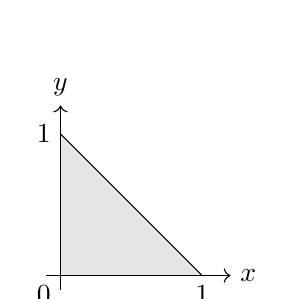
\begin{tikzpicture}[scale=1.8]
\fill[gray!20] (0,0)--(1,0)--(0,1)--cycle;
\draw[->](-.1,0)--(1.2,0)node[right]{$x$};
\draw[->](0,-.1)--(0,1.2)node[above]{$y$};
\draw(0,1)--(1,0);\node[below left]at(0,0){$0$};
\node[below]at(1,0){$1$};\node[left]at(0,1){$1$};
\end{tikzpicture}
\end{center}
Normalization gives
\[
1=\int_0^1\int_0^{1-x}cx^3y\d y\d x
=c\int_0^1x^3\frac{(1-x)^2}2\d x=\frac c{120},
\qquad c=120.
\]
The marginal density is
\[
f_X(x)=\int_0^{1-x}cx^3y\d y=cx^3\frac{(1-x)^2}2,
\qquad x\in[0,1],
\]
and
\begin{align*}
\E Y&=\int_0^1\int_0^{1-x}y\,cx^3y\d y\d x\\
&=c\int_0^1x^3\frac{(1-x)^3}3\d x
=\frac{120}{420}=\frac27\approx0.2857.
\end{align*}
\subsection*{(b) Conditional expectations}
Clearly, $\E[X\mid X=1/2]=1/2$. Also,
\[
\E[Y\mid X=1/2]
=\int_0^{1/2}y\frac{c(1/2)^3y}{c(1/2)^3(1/2)^2/2}\d y
=8\int_0^{1/2}y^2\d y=\frac13.
\]
\subsection*{(c) The product}
Set $Z=XY$ and $W=X$. Then $X=W$, $Y=Z/W$ and
\[
\det J=\begin{vmatrix}0&1\\1/w&-z/w^2\end{vmatrix}=-\frac1w.
\]
Consequently,
\begin{align*}
f_{Z,W}(z,w)&=f_{X,Y}(w,z/w)\frac1{|w|}\\
&=cw^3\frac zw\frac1w\mathbf1_{\{w+z/w\le1,\ z,w\ge0\}}
=czw\mathbf1_{\{z,w\ge0,\ z\le w-w^2\}}.
\end{align*}
The condition is $w^2-w+z\le0$, whose roots are
\[
w_{1,2}=\frac{1\mp\sqrt{1-4z}}2.
\]
Thus $0\le z\le1/4$ and $w$ lies between these roots. Integrating,
\begin{align*}
f_Z(z)&=\int_{(1-\sqrt{1-4z})/2}^{(1+\sqrt{1-4z})/2}czw\d w\\
&=\frac{cz}{8}\left[(1+\sqrt{1-4z})^2-(1-\sqrt{1-4z})^2\right]\\
&=\frac{cz}{8}\,4\sqrt{1-4z}=\frac{cz\sqrt{1-4z}}2,
\qquad z\in[0,1/4].
\end{align*}

\section*{Problem 3}
\subsection*{(a) Red cells}
Let $X$ be the number of red cells, so $X\sim\operatorname{Bin}(81,1/3)$. Then
\[
\P(X\le21)=\P\left(\frac{X-81/3}{\sqrt{81\cdot\frac13\cdot\frac23}}
\le\frac{21-81/3}{\sqrt{81\cdot\frac29}}\right)
\approx\Phi(-1.41)\approx7.93\%,
\]
using the central limit theorem (why is it applicable?).
\subsection*{(b) Flags}
No: possible flag positions overlap. Think about a formal proof!
\subsection*{(c) Expected number of flags}
The possible positions are $7$ per row times $9$ rows. Number them. If $X_i$ is the indicator that position $i$ contains a flag, then $X_i\sim\operatorname{Ber}(1/27)$. The source writes
\[
\E[\text{number of vertical flags}]
=\E[X_1+\cdots+X_{67}]=67\E X_1=\frac{67}{27}.\tag{Note 2}
\]
\subsection*{(d) Both orientations}
They are not independent (why?). By linearity, the original concludes
\[
\E[\text{vertical}+\text{horizontal}]
=2\E[\text{vertical}]=\frac{134}{27}.\tag{Note 2}
\]

\section*{Problem 4}
\subsection*{(a) Sums of exponentials}
By convolution,
\[
f_{X+Y}(x)=\int_{-\infty}^\infty f_X(y)f_Y(x-y)\d y.
\]
Hence, for $x\ge0$,
\[
f_{S_2}(x)=\int_{-\infty}^\infty e^{-y}e^{-(x-y)}
\mathbf1_{\{y,x-y\ge0\}}\d y
=\int_0^xe^{-x}\d y=xe^{-x}.
\]
For the induction, the source labels the preceding density
$f_{S_{n-1}}(x)=x^{n-1}e^{-x}\mathbf1_{\{x>0\}}/(n-1)!$
and writes
\begin{align*}
f_{S_n}(x)&=\int_{-\infty}^\infty\frac{y^{n-1}}{(n-1)!}
e^{-y}e^{y-x}\mathbf1_{\{y,x-y\ge0\}}\d y\\
&=e^{-x}\int_0^x\frac{y^{n-1}}{(n-1)!}\d y
=\frac{x^n}{n!}e^{-x}\mathbf1_{\{x>0\}}.\tag{Note 3}
\end{align*}
\subsection*{(b)} $\ldots$
\subsection*{(c) The counting variable}
\begin{align*}
\P(N_t=n)&=\P(S_n\le t)-\P(S_{n+1}\le t)\\
&=\int_0^t\frac{x^{n-1}}{(n-1)!}e^{-x}\d x
-\int_0^t\frac{x^n}{n!}e^{-x}\d x.
\end{align*}
Integration by parts gives
\[
\int_0^t\frac{x^n}{n!}e^{-x}\d x
=\left[-\frac{x^n}{n!}e^{-x}\right]_0^t
+\int_0^te^{-x}\frac{x^{n-1}}{(n-1)!}\d x.
\]
The repeated integrals cancel, yielding
\[
\P(N_t=n)=e^{-t}\frac{t^n}{n!}.
\]
The source's final boxed statement is $N_t\sim\operatorname{Poi}(1)$. See Note 4.

\section*{Transcription notes}
\begin{enumerate}
\item The variance expression for $Z_1$ is approximately $34.08$, not $1225.97$. The source carries its stated value into the five-bet variance as well.
\item The source states $7\cdot9$ positions but uses 67 in the subsequent count. There are 63 positions for either orientation, so the displayed expectations require review.
\item The induction labels are shifted: the density $x^{n-1}e^{-x}/(n-1)!$ belongs to $S_n$ and its convolution with an additional exponential belongs to $S_{n+1}$.
\item The displayed probability mass function has Poisson parameter $t$. The source's final parameter 1 is inconsistent with that mass function.
\end{enumerate}
\end{document}
